
\chapter{实验测试与结果分析}

\section{实验环境与测试负载}

\subsection{硬件配置}

\subsection{实验环境选择说明}

本研究涉及对Linux内核的深度修改与定制,实验环境的选择受到多种因素的限制。首先,由于对内核进行了大量底层改动,测试环境需要完全控制系统底层权限并能够频繁重启以更新内核,而生产环境不允许此类操作;其次,修改后的内核需要经过充分验证才能部署到高端服务器上,以避免潜在的系统稳定性问题。因此,本研究采用了性能较为有限的笔记本电脑作为测试平台,虽然测试平台的绝对性能与企业级服务器存在差距,但本研究关注的是不同算法间的相对性能比较,以及算法在不同工作负载下的适应性表现,这些方面的结论在很大程度上可以推广到更高性能的硬件环境中。未来研究中,在核心算法稳定后,可考虑在大规模服务器集群上进行进一步验证。

表\ref{tab:hardware_config}汇总了实验平台的具体配置,可以看到该平台拥有 Intel(R) Core(TM) i7-8750H CPU @ 2.20GHz 以及 16GB DDR4 内存。为了在内核中进行对比,本研究分别选取了机械硬盘、SSD 和 zram 这三种不同的卸载后端。之所以进行这样的选择,一方面是由于官方内核暂未实现基于 RDMA 和 NVM 的卸载后端,另一方面也是为了更好地体现不同存储介质在 I/O 延迟和读写性能方面的差异。机械硬盘能够代表最传统、也是性能相对最差的卸载方式,SSD 在随机读写和延迟方面有一定程度提升,而 zram 则具有数据压缩和低延迟的优势,通常被认为是内存交换的优先方案。为了凸显 zram 的潜在优势,并评估自适应算法在高压缩比数据下的实际效果,本文在后续测试中也将 zram 视为可获得最优 I/O 性能的后端加以重点分析。

\begin{table}[ht]
    \centering
    \caption{实验平台硬件配置}
    \label{tab:hardware_config}
    \begin{tabular}{ll}
        \toprule
        CPU & Intel(R) Core(TM) i7-8750H @ 2.20GHz \\
        \midrule
        Memory & 16GB (2 \(\times\) 8GB) DDR4 @ 2667MT/s SODIMM \\
        \midrule
        SSD & Intel SSDPEKKW256G8 NVMe SSD (256GB, PCIe Gen3 x4)  \\
        \midrule
        HDD & Seagate ST1000LM035 HDD (1TB, 5400 RPM) \\
        \bottomrule
    \end{tabular}
\end{table}

在负载选择方面,为了更全面地测试本文提出方案的通用性,实验分别使用了文件密集型的 Web Server 和内存密集型的 Redis 这两类典型应用。Web Server 场景主要用于观察系统针对大量静态文件(包括高清图片与文本数据)缓存时的文件页回收策略,而 Redis 场景则聚焦在匿名页占比极高的内存回收状态。值得注意的是,在 Redis 测试中禁止了持久化功能并关闭了淘汰策略,这样能更直接地暴露内存回收在内核层面的有效性,因为一旦允许用户态自行管理持久化或淘汰,就会在应用层与内核层产生额外耦合,从而干扰对回收策略的评估。

\section{模块功能与有效性测试}

\subsection{内存压力模块有效性验证}

在展开具体算法评估之前,需要首先验证所设计的内存压力模块能否在不借助用户态复杂逻辑的前提下,为系统施加可量化的内存压力。为此,本文使用了 Web Server 作为负载,将各种类型的图片和文字文件提前放入服务器端,随后利用压力发生器随机并持续地发起请求,同时在内核中分别配置机械硬盘、SSD 和 zram 作为卸载后端。通过这样的方式,可以从 16GB 可用内存开始,逐步减少可用空间直到 6GB,借此形成多轮测试,并观察在不同后端介质下系统对内存压力的响应程度。图\ref{fig:memory_pressure}展示了三种卸载后端下的内存压力曲线。可以明显看出,机械硬盘由于读写延迟和带宽的劣势,会更频繁地陷入换入换出操作,导致系统大量时间都处在高压力区间,甚至难以稳定地对外提供请求服务;相比之下,SSD 提供了更快的 I/O 响应能力,zram 在具有压缩和低访问延迟的双重优势下,则能进一步缓解内存压力飙升的问题。通过该实验可以确认本研究的内存压力模块在不同后端下均能触发与还原高压场景所需的换页流程,且能够准确地量化系统内存使用状况,为后续的自适应回收算法测试奠定基础。

\begin{figure}[htbp]
    \centering
    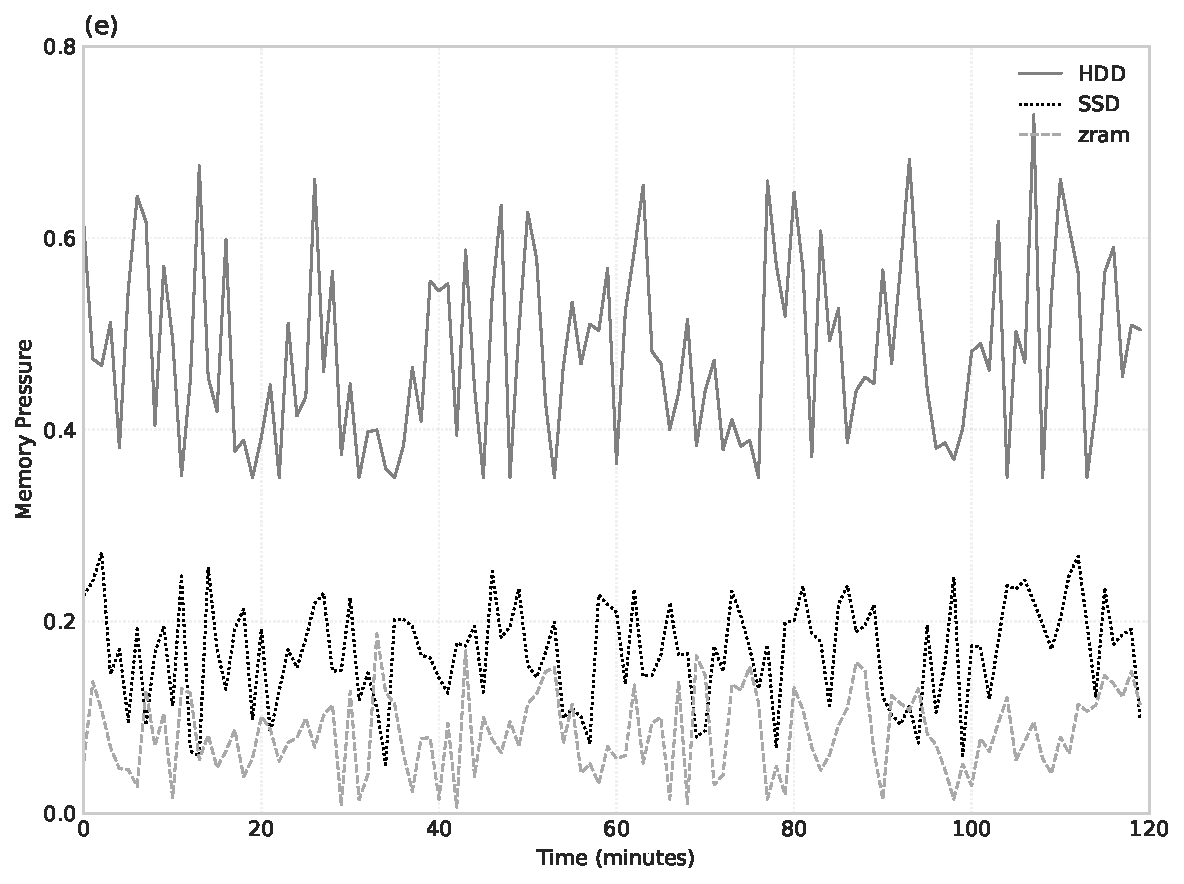
\includegraphics[width=\textwidth]{memory_pressure.pdf}
    \caption{三种卸载后端下的内存压力对比}
    \label{fig:memory_pressure}
\end{figure}


\subsection{文件页与匿名页均衡算法有效性验证}
\label{sec:file_page_anonymous_page_balance_algorithm_validation}

在确认内存压力模块可以生成可控且真实的压力环境后,需要检验自适应回收算法的第二个核心:即针对文件页与匿名页的均衡回收机制。为此,本文选取了 10GB 的可用内存作为上限来运行高负载场景,并针对 Linux 内核中的  swappiness  参数进行多轮对比测试。实验中分别测试了使用默认内核策略(baseline)和启用自适应均衡算法(adaptive  swappiness)两种情况下的系统性能表现。

\begin{figure}[htbp]
    \centering
    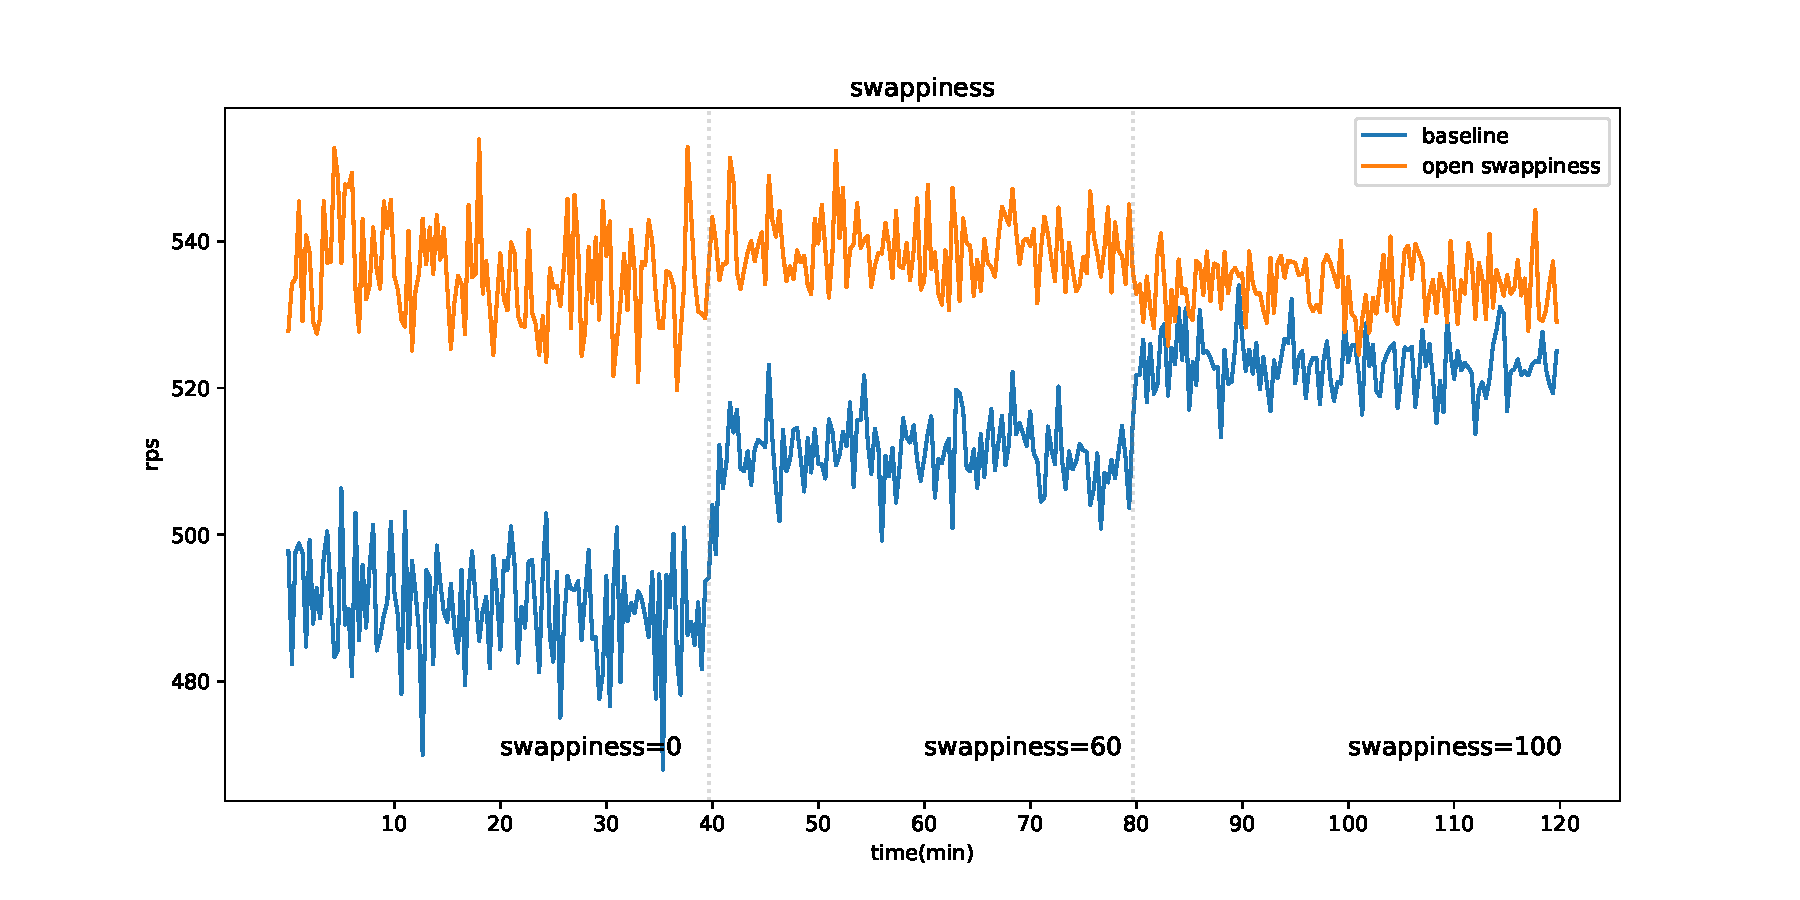
\includegraphics[width=\textwidth]{swappiness.pdf}
    \caption{Web Server 在不同  swappiness  下的性能变化}
    \label{fig:web_server_swappiness}
\end{figure}

首先在文件密集型负载(Web Server)下进行测试,如图\ref{fig:web_server_swappiness}所示。在默认内核策略下,当  swappiness =0 时,系统优先回收文件页而保留匿名页,导致Web Server所需的文件缓存被频繁驱逐,平均RPS仅维持在490左右;当  swappiness  提升至 60 时,系统开始更均衡地回收文件页和匿名页,使得Web Server的关键文件缓存得到一定保留,RPS明显提升至约515;进一步将 swappiness 提高到100时,RPS继续小幅上升至520左右,但增幅已不显著,这表明在文件密集型负载下,适当提高匿名页回收比例能有效改善系统性能。

当启用自适应均衡算法后,其性能表现更为优异。图中橙色曲线显示,无论 swappiness 设置为何值,系统吞吐量均维持在535-540之间的较高水平,且波动较小。特别是在 swappiness =0的情况下,相比默认策略提升了约10\%的吞吐量,这证明了算法能够准确识别频繁访问的文件页,并通过动态调整回收策略避免了过度驱逐热文件页的问题。

\begin{figure}[htbp]
    \centering
    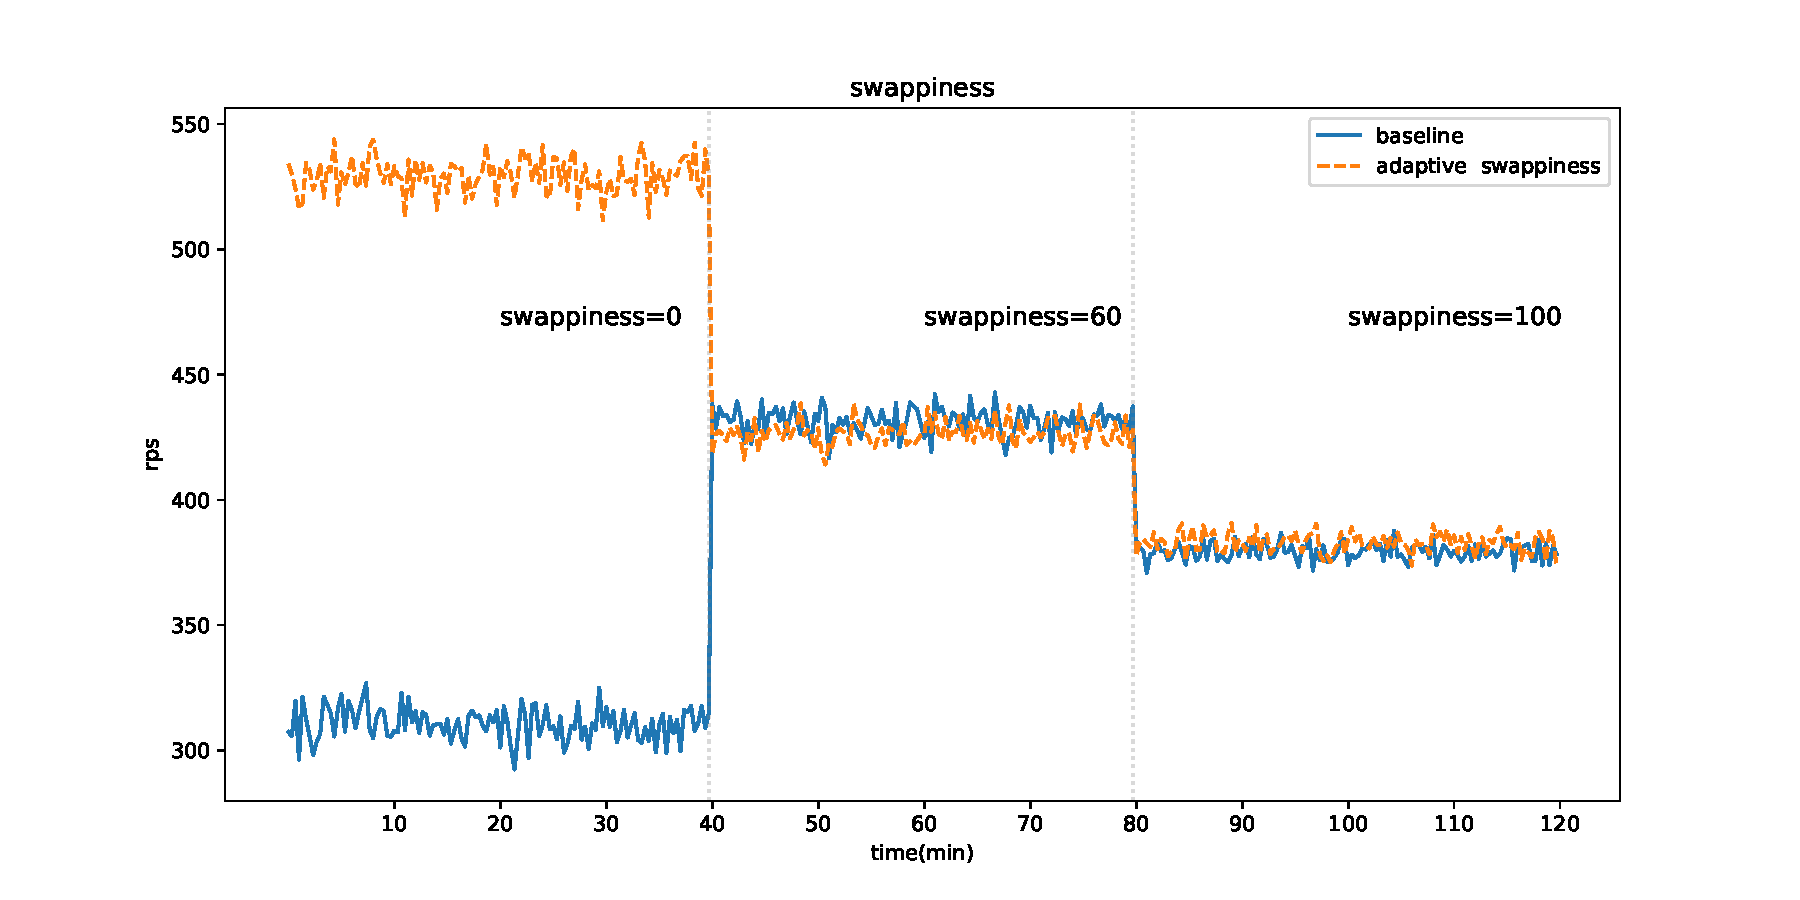
\includegraphics[width=\textwidth]{redis_swappiness.pdf}
    \caption{Redis 在不同  swappiness  下的性能变化}
    \label{fig:redis_swappiness}
\end{figure}

为验证算法在不同类型工作负载下的适应性,本文进一步选取了Redis作为内存密集型测试对象。如图\ref{fig:redis_swappiness}所示,Redis测试展现出了与Web Server截然不同的性能特征。在默认内核策略下, swappiness =0时Redis的平均RPS仅为310左右;当提高至 swappiness =60后,RPS骤增至430左右;而进一步提高至 swappiness =100时,性能又下降至380左右。这一曲线变化表明,在匿名页占主导的Redis工作负载中,过低的 swappiness 值会导致系统几乎不回收匿名页,使得内存压力集中在文件页上,而这些文件页可能包含程序代码等关键部分;适度提高 swappiness 可以实现更均衡的回收策略;但过高的值则会导致过度回收匿名页,引发频繁的页面换入换出。

当启用自适应均衡算法后,系统表现出更强的环境适应能力。在 swappiness 为0的配置下,启用算法的Redis性能(约525 RPS)显著优于默认策略,远高于任何 swappiness 值下的默认策略表现。这表明算法能够通过分析页面访问模式,自动调整回收策略,避免了在内存紧张时对程序关键文件页的错误驱逐。在 swappiness =60和100的配置下,启用算法后的性能与默认策略相近,这是因为在Redis这类匿名页占比极高(约90\%)的场景中,文件页缺页率相对较低,算法优化空间有限。

实验结果表明,本文提出的文件页与匿名页均衡算法在不同类型的工作负载下均能展现良好适应性。在文件密集型负载中,算法能够通过精确识别热文件页并保留它们来提升性能;在内存密集型负载中,算法也能避免关键文件页被错误驱逐。虽然在极高匿名页占比的环境中算法的优化空间相对有限,但这也符合内存管理的理论预期,因为当工作集几乎完全由匿名页构成时,页面类型差异化回收的影响自然会降低。通过这两类代表性应用的实验,初步验证了该算法具有较强的通用适应能力。

\section{综合测试}

\subsection{测试目标}

上述实验分别验证了内存压力模块在不同后端介质下的量化能力,以及文件页与匿名页均衡算法在不同类型工作负载下的适应性。为了更深入地了解将二者结合起来后对系统整体性能和资源使用的影响,本文设计了综合测试。该测试主要聚焦以下问题:在持续提供服务的高负载场景下,若开启自适应算法并在不同后端(SSD 与 zram)进行内存卸载,系统能否稳定提升吞吐量并节约内存占用;在用户态应用(如 Web Server)长期占用大规模文件页以及针对容器化的多进程场景下,算法是否依旧有良好的适应性。

\subsection{测试方案}

首先在 Web Server 场景下,通过一轮预热请求将常见的文件页面基本加载至内存中,以形成完整的工作集,然后维持高并发请求并逐步向系统注入额外的内存压力,依次在以下场景下进行对比:(1) 禁用  swap ;(2) 启用  swap  并使用 SSD;(3) 启用  swap  并使用 zram;(4) 在(2)与(3)基础上额外启用自适应算法(含内存压力模块、文件页与匿名页均衡及基于压力的工作集评估)。为量化效果,本文重点记录并分析 RPS、系统内存使用量、缺页中断次数(refault)以及 p90 响应时间等关键指标,结合曲线变化对整体性能加以解释。

\subsection{测试结果与分析}
\label{sec:test_result}

图\ref{fig:rps}、图\ref{fig:mem}、图\ref{fig:refault}和图\ref{fig:p90}汇总了本研究的主要观测指标,包括系统吞吐量、内存使用、缺页中断次数及 p90 事务响应时间。通过对比可发现,禁用  swap  的基准方案一开始或许能获得更高的 RPS,但随着负载不断累积,内存在无外部卸载路径的情况下很快就会达到饱和并导致性能显著下滑。当启用 SSD  swap  或 zram  swap  时,系统能够将一部分冷门页面换出,维持一定程度的内存空间,但在默认策略下并不能总是准确地识别哪些页面应该被回收,因此会出现阶段性波动。当在  swap  基础上启用自适应算法后,系统性能显著稳定:SSD 场景能保持近乎平稳的 RPS,zram 场景则在其更优的压缩和 I/O 特性加持下,使最终吞吐量略有进一步的上升。

\begin{figure}[htbp]
    \centering
    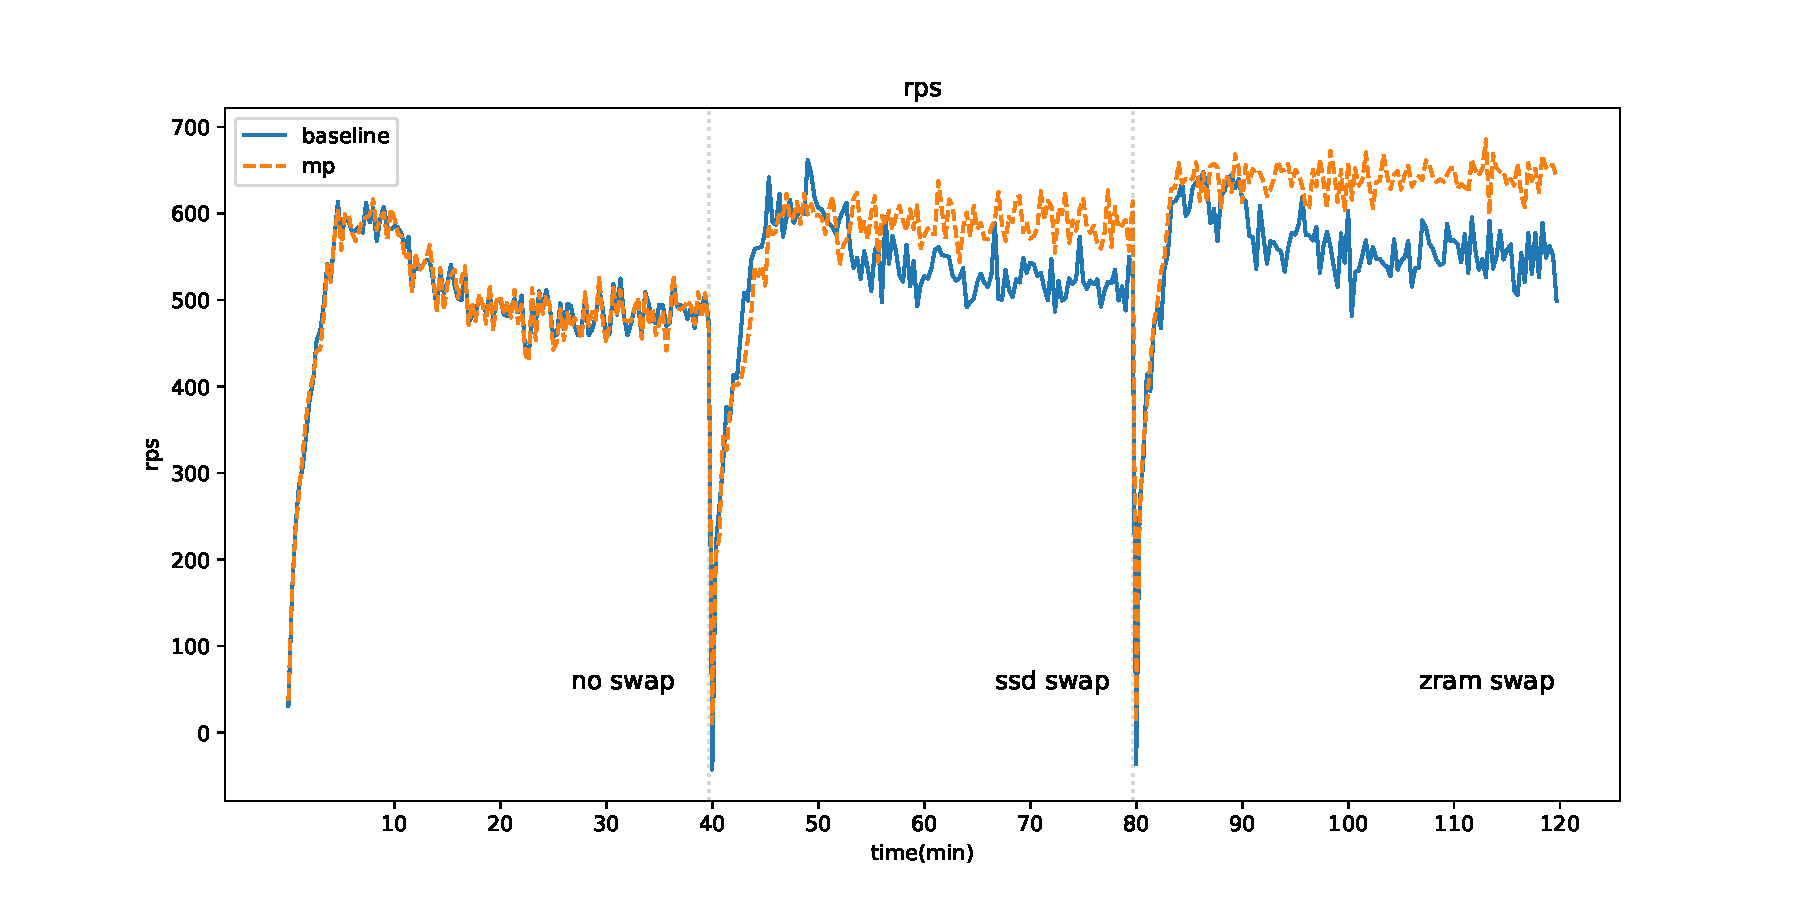
\includegraphics[width=\textwidth]{rps.pdf}
    \caption{Web Server 负载在多种场景下的 RPS 对比}
    \label{fig:rps}
\end{figure}

从内存使用角度而言,图\ref{fig:mem}展示了不同时刻系统实际占用的内存空间。禁止  swap  时的占用最为紧张,一旦工作集超出物理可用范围,性能会大幅波动。SSD  swap  能在一定程度上释放物理内存,但幅度有限;zram 则借助压缩手段使得内存占用有明显下降。若配合自适应回收算法,系统会更积极地识别低频访问页面,并在合适时机将其卸载,从而在相同负载下保持更低的物理内存占用。值得强调的是 zram 场景的差异更为显著,说明当卸载后端访问成本较低时,内核会更加大胆地进行页面回收,以换取主内存空间的可用度。

\begin{figure}[htbp]
    \centering
    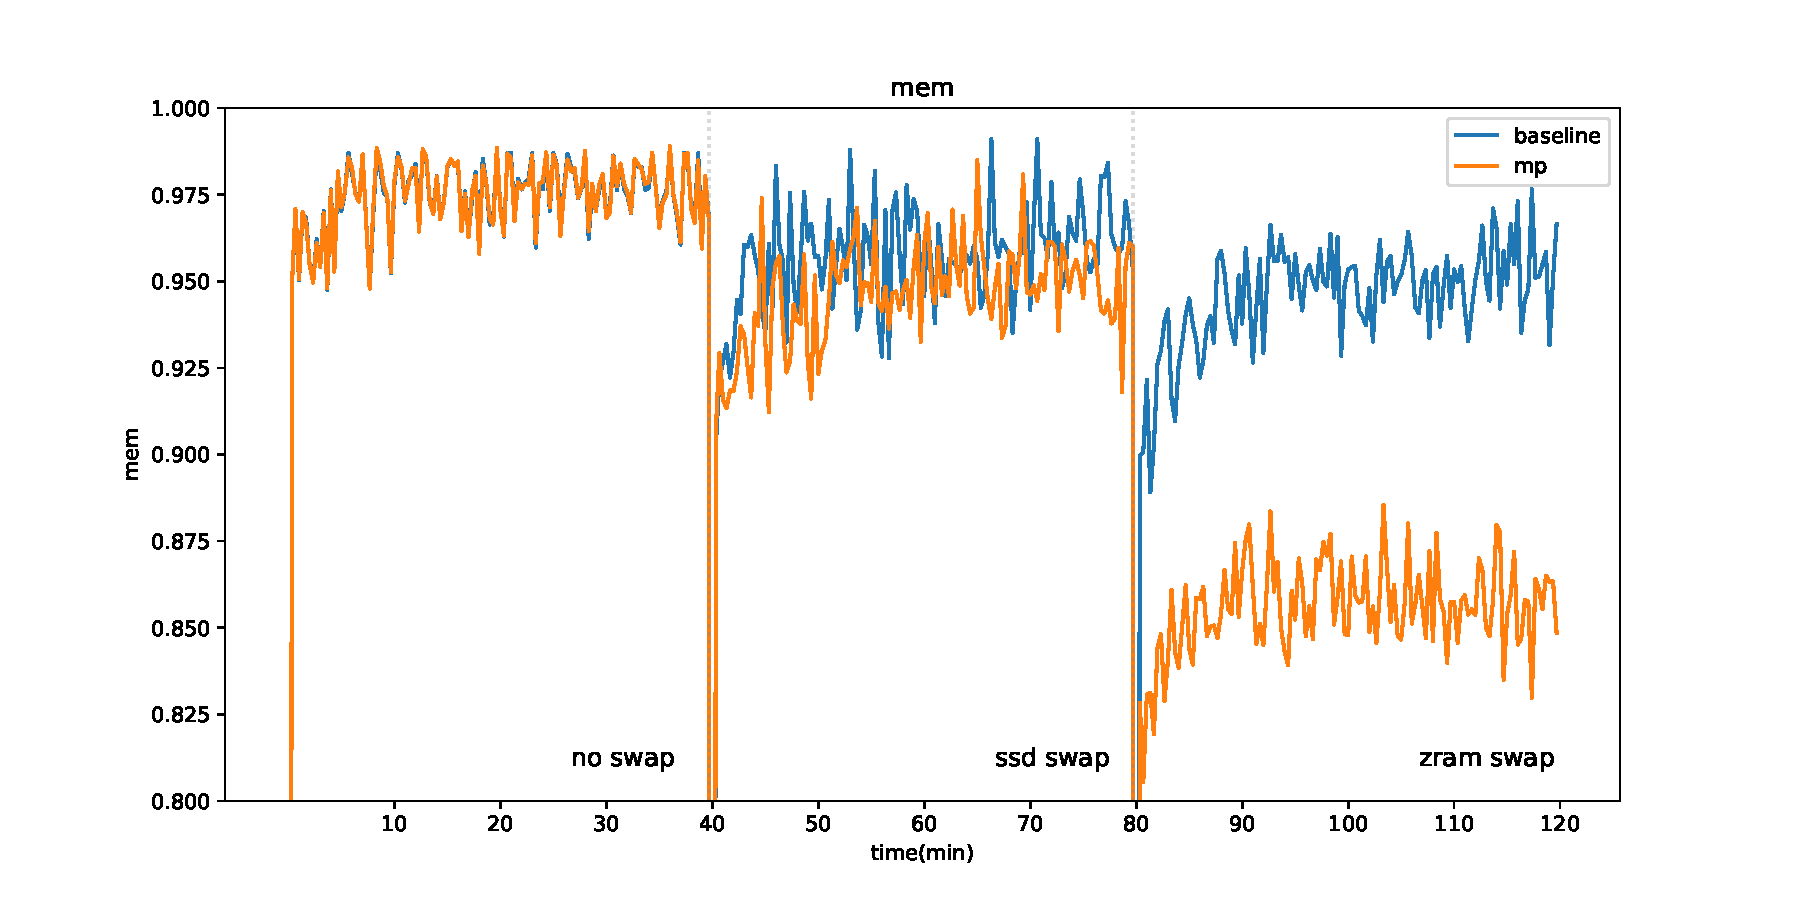
\includegraphics[width=\textwidth]{mem.pdf}
    \caption{Web Server 负载在多种场景下的内存使用对比}
    \label{fig:mem}
\end{figure}

在缺页中断次数方面,图\ref{fig:refault}显示了随着时间推移不同  swap  策略下的 refault 变化。zram 由于读写延迟远小于机械硬盘或常规 SSD,系统在侦测到其性能优势后往往会更积极地回收页面,一旦后续访问到已被回收的页面便会触发缺页中断,于是 zram 场景的 refault 次数偏高。表面上看这似乎意味着更多的页面换入操作,但其实际代价因为 zram 极低的访问延迟而相对有限,因此并不会对系统吞吐形成严重拖累。

p90 响应时间如图\ref{fig:p90}所示,能够比较直观地体现系统在尾部延迟上的表现。可以看到在 SSD 作为卸载后端时,由于其 I/O 性能虽优于 HDD 但依旧是一个相对独立的外部存储介质,随机小块读写性能不及压缩内存,p90 相对略高且更易抖动;而 zram 场景在高压缩比与高吞吐特性下,能将尾部延迟维持在一个更低且更稳定的水平。当结合自适应算法后,zram 场景的 p90 再度下降,说明该算法可以及时识别并淘汰不活跃页面,从而降低了频繁换入对关键请求导致的尾部延迟。

\begin{figure}[htbp]
    \centering
    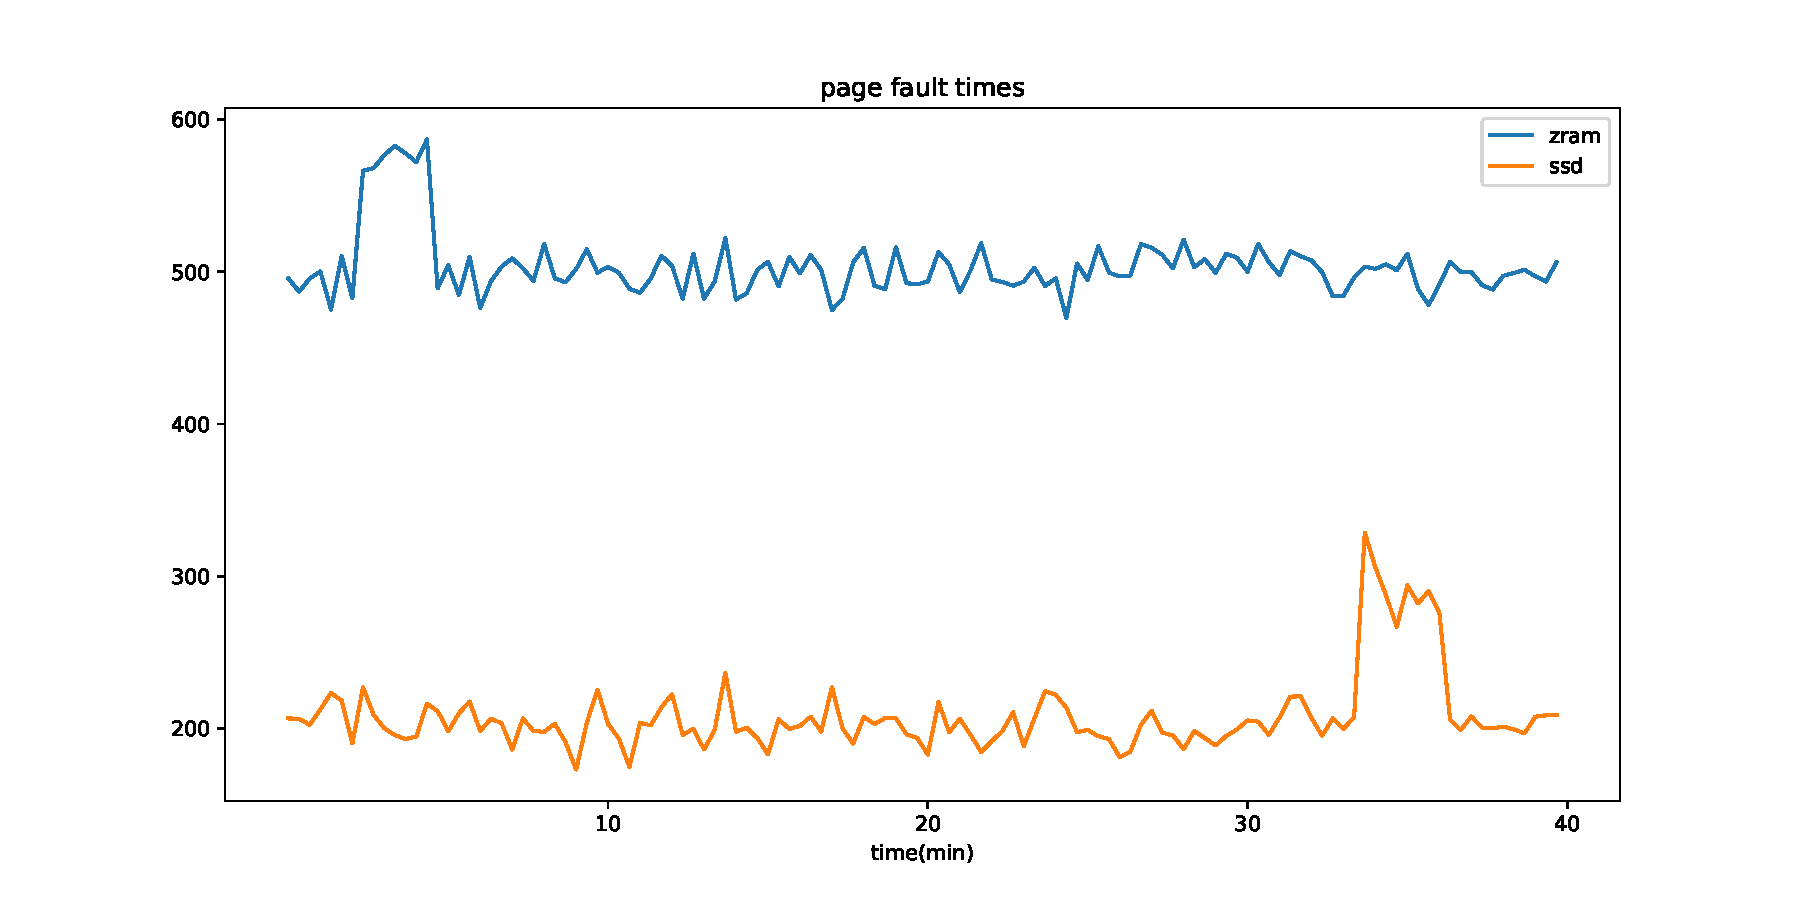
\includegraphics[width=\textwidth]{refault.pdf}
    \caption{Web Server 负载在多种场景下的缺页中断次数}
    \label{fig:refault}
\end{figure}



\begin{figure}[htbp]
    \centering
    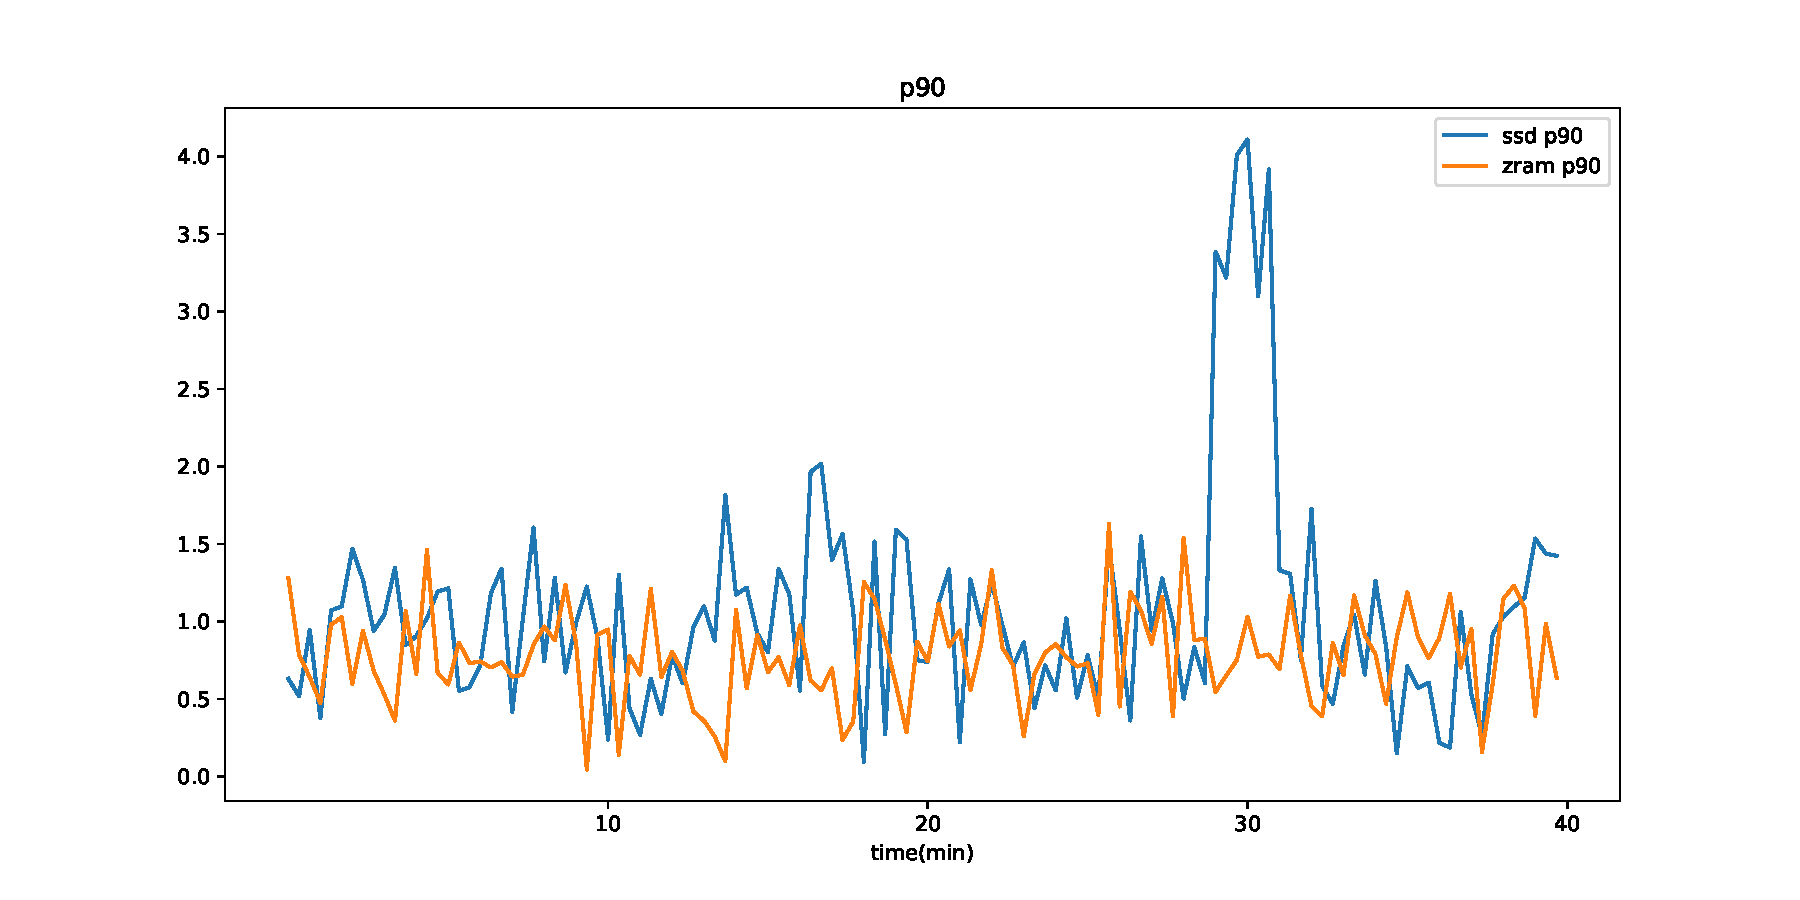
\includegraphics[width=\textwidth]{p90.pdf}
    \caption{Web Server 负载在多种场景下的 p90 响应时间对比}
    \label{fig:p90}
\end{figure}

最后,图\ref{fig:container_memory}展示了容器化场景下的实验结果,特别关注了当 Kubernetes 或类似系统为每个 Pod 创建顶层 CGroup 并在其中运行边车容器与业务容器时,整体内存使用的变化。随着容器数量规模的增长,边车容器在日志、流量代理和监控探针等方面产生的“虚拟化税”累积效应会日益突出。本研究在容器环境中同样利用内存压力模块与自适应回收算法对边车容器和核心负载容器进行同时检测,实测表明边车容器中相当一部分页面实际上是低频或不活跃数据,卸载到高性能介质(尤其是 zram)后可有效释放物理内存,从而将更多主内存资源留给核心负载,增强了集群整体的资源利用率与稳定性。

\begin{figure}[htbp]
    \centering
    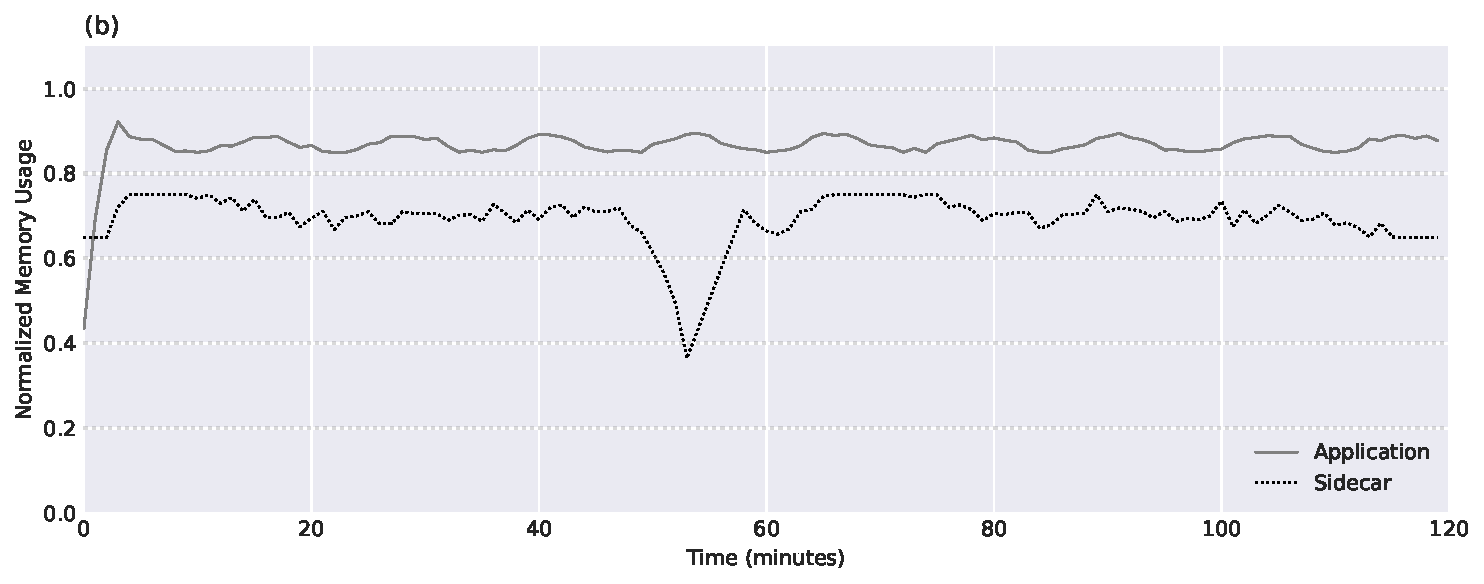
\includegraphics[width=\textwidth]{container_memory.pdf}
    \caption{自适应算法在边车容器与业务容器中的内存释放效果对比}
    \label{fig:container_memory}
\end{figure}

\section{本章小结}

通过本章一系列实验,可以得出以下主要结论:首先,本文所设计的内存压力模块能够在机械硬盘、SSD 和 zram 这三种卸载后端下有效触发和量化系统的内存压力,为后续回收算法提供真实的环境支撑。其次,文件页与匿名页均衡算法在文件密集型和内存密集型负载中均展现出良好的适用性,其针对  swappiness  的动态调节可避免过度回收缓存文件页或引发过度的匿名页换入换出,从而在不同场景里带来显著性能增益。再次,在综合测试中,结合内存压力与自适应均衡的整体方案能够高效地释放物理内存并在高负载时保持稳定的吞吐和延迟表现,其中 zram 作为卸载后端时展现了更加出色的性能。最后,在容器化场景下,边车容器的内存占用常常在实际部署中造成可观的资源浪费,通过在内核中实施基于压力的自适应回收机制,能够大幅降低这部分“虚拟化税”,在大规模服务环境下具有突出的应用价值。上述结论为下一步在更复杂或更大规模生产环境中推广这一内存回收与卸载方案提供了重要参考依据。
